\documentclass[12pt]{article}

\usepackage{sbc-template}

\usepackage{graphicx,url}
 
\usepackage[utf8]{inputenc}
\usepackage{holtxdoc}
\usepackage{hyperref}
\usepackage{lstdoc}
\usepackage{minted}



\hypersetup{
    colorlinks=true,      % ativa as cores dos links
    linkcolor=black,       % cor dos links internos
    urlcolor=black,        % cor dos links externos
    citecolor=black        % cor das citações
}


\lstset{
    language=C,                        % Linguagem de programação
    basicstyle=\ttfamily\footnotesize, % Fonte do código
    keywordstyle=\color{blue},         % Cor das palavras-chave
    stringstyle=\color{green!60!black},% Cor das strings
    commentstyle=\color{gray},         % Cor dos comentários
    numbers=left,                      % Números das linhas à esquerda
    numberstyle=\tiny\color{gray},     % Estilo dos números das linhas
    stepnumber=1,                      % Intervalo entre números das linhas
    breaklines=true,                   % Quebra automática de linha
    frame=single,                      % Moldura ao redor do código
    tabsize=4,                         % Tamanho do tab
    captionpos=b,                      % Posição da legenda (b = abaixo)
    showspaces=false,                  % Não mostra espaços com sublinhados
    showstringspaces=false,            % Não mostra espaços em strings
    morekeywords={printf, scanf},      % Palavras-chave adicionais
}


     
\sloppy

\title{TSO - 2024.2 - JOÃO PEDRO FERREIRA DUARTE}

\author{João Pedro F. Duarte\inst{1} }

\address{Bacharelado em Engenharia de Computação\\
Centro Federal de Educação Tecnológica de Minas Gerais (CEFET-MG)\\
   Minas Gerais -- MG -- Brasil
  \email{\ joaopedrofduarte@outlook.com}
}

\begin{document} 

\maketitle

\section{Implementação da Syscall no SO Minix3}

\begin{abstract}
    In Operating Systems, system calls, \texttt{Syscalls}, are functions renewed to perform some type of specific service in favor of the processes carried out by the OS.
    With this same objective, the present study presents the implementation of a \texttt{Syscall}, which we will call \textbf{useless}, within the Minix3.2.1 Process Manager Server, for purposes
    study on this process.
\end{abstract}
     
\begin{resumo}
Em Sistemas Operacionais, chamadas de sistema, \texttt{Syscalls}, são funções implementadas para realizar algum tipo de serviço específico em favor dos processos realizados
pelo SO. Com este mesmo objetivo, o presente estudo apresenta a implementação de uma \texttt{Syscall}, que a chamaremos de \textbf{inútil}, dentro do Servidor Gerenciador de
Processo do Minix3.2.1, para fins de estudo sobre este processo.
\end{resumo}


\subsection{Introdução} %Configuracoes e ambiente

O presente texto, com objetivo de instriução, serve para que qualquer programados com o intuito de estudar mais sobre os conceitos relacionados a Sistemas Operacionais
, através do uso do Minix, em sua versão $3.2.1$, possa realizar todos os passos necessários para implementar, desde o início, a criação de uma chamada de sistema. Em
maiores detalhes, temos aqui as referências \cite{creating_syscall} e \cite{tanenbaum_modern_os} como fontes base para entendimento do Kernel do sistema operacional em uso,
como também da documentação presente no site do Minix para desenvolvedores conforme \cite{minix3docs}. \href{https://www.minix3.org/doc/}{Link da documentação}.
%

Sobre a ambientação necessária para o desenvolvimento deste projeto, o programador deve realizar a instalação de uma máquina virtual minix, na versão correta para este projeto
e realizar todas as etapas de instalação do sistema operacional conforme documentação oficial supracitada. O link referente à plataforma onde deve ser criada a máquina virtual,
como também ao local onde estará a versão correta do sistema operacional e a parte da documentação onde constam as etapas de instalação do sistema, podem ser consultados a seguir:
\href{https://www.virtualbox.org/wiki/Downloads}{[Virtual Box]}, \href{https://wiki.minix3.org/doku.php?id=www:download:start}{[Minix versão 3.2.1]} e \href{https://wiki.minix3.org/doku.php?id=usersguide:runningonvirtualbox}{[processo de instalação]}.


\subsection{Primeiro caso} \label{sec:1sec}
Inicialmente, para dar início ao processo de criação da chamada de sistema, tem-se como focos de alteração e estudo para fins de entendimento do processo interno do
Kernel do sistema operacional, a aplicação das seguintes rotas para atualização de dados e manipulação.

\begin{enumerate}
    \item \label{callnr} /callnr.h: Aqui está a listagem de todas as chamadas de sistema presentes no Minix.
    \item  \label{table} /table.c: Aqui estão os nomes de cada uma das rotinas das chamadas de sistema do Minix.
    \item  \label{proto} /proto.h: Protótipo de todas as rotinas de chamadas de sistema do sistema operacinal.
    \item  \label{misc} /misc.c: Chamada de sistema de todas as Syscalls do tipo \texttt{Misc}.
    \item  \label{minhachamadalib} /minhachamadalib.h: Este é o "include file" que realiza a chamada da chamada de sistema \texttt{inútil}.
    \item  \label{teste1} /teste1.c: Arquivo de teste criado para realizar o teste da chamada \texttt{inútil}.
\end{enumerate}

Para realizar a manipulação dos diretórios, de forma a acessar, listar, ver conteúdo, editar e salvar arquivos, pode-se usar comandos Linux padrão, conforme pode ser
cultado em \href{https://www.devmedia.com.br/comandos-importantes-linux/23893}{[Lista de comandos básicos pela DevMedia]}.

\subsection{Segundo Caso} \label{sec:2sec}
O primeiro passo da atividade consiste em acessar o arquivo \ref{callnr} através do comando \texttt{vi}, em \lstinline{/usr/src/include/minix/callnr.h}, assim, através do comando
\lstinline{vi /usr/src/include/minix/callnr.h}. Neste arquivo, deve ser inserida as seguinte linha entre as chamadas de sistema $68$ e $71$. \lstinline{# define MYSYSCALL 69}.
Após realizar a inserção do valor na linha, basta salvar o arquivo e sair do editor de texto \texttt{vi}, através do comando \lstinline{wq}. O arquivo referenciado pode ser visto
abaixo na figura \ref{fig1}.

\begin{figure}[htbp]
    \centering
    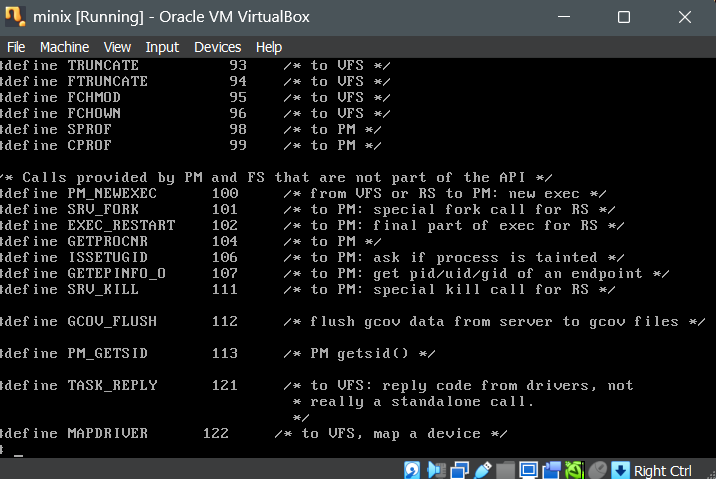
\includegraphics[scale=0.6]{out/fig/Screenshot 2024-12-23 112211}
    \caption{Caminho de referência de \texttt{callnr.h}.}
    \label{fig1}
\end{figure}

\subsection{Terceiro Caso} \label{sec:3sec}
Agora é necessário navegar até \ref{table} através do comando \lstinline{vi}, que permita a abertura do editor do arquivo. Procure neste arquivo pela seguinte linha:
\lstinline{no_sys, /* 69 = unused */}, e nesta mesma linha, faça a substituição do conteúdo por \lstinline{do_mysyscall, /* 69 = my sys call */}. O caminho completo para este
acesso é \lstinline{vi /usr/src/servers/pm/table.c}

\begin{figure}[htbp]
    \centering
    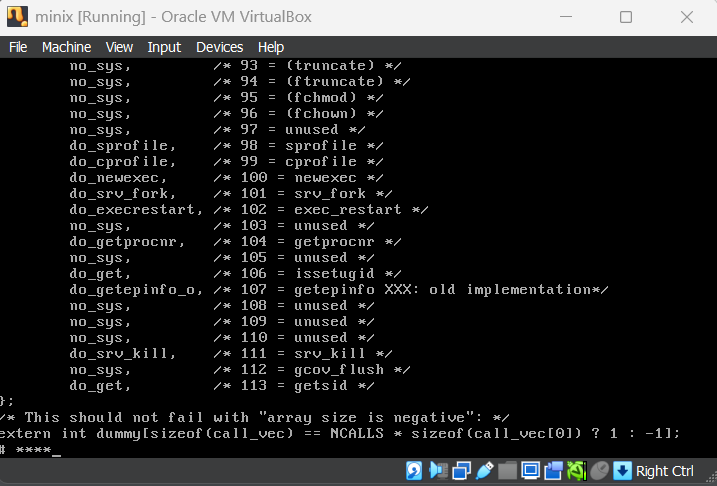
\includegraphics[scale=0.6]{out/fig/Screenshot 2024-12-23 151307}
    \caption{Caminho de referência de \texttt{table}.}
    \label{fig3}
\end{figure}

\subsection{Quarto Caso} \label{sec:4sec}

Como terceira etapa do processo de criação da chamada de sistema, agora é necessário navegar com o comando \lstinline{vi} e abrir o arquivo \ref{proto}, através da instrução
\lstinline{vi /usr/src/servers/pm/proto.h}. Aqui, devemos procurar pela linha \lstinline{int do_getsetpriority(void); (inside /* misc.c */)} e realizar a adição, uma linha acima da já referida
linha, a seguinte função, \lstinline{int do_mysyscall(void);}. Dada finalização da edição, basta agora, assim como anteriormente, salvar e sair do presente arquivo por \lstinline{wq}.

\begin{figure}[htbp]
    \centering
    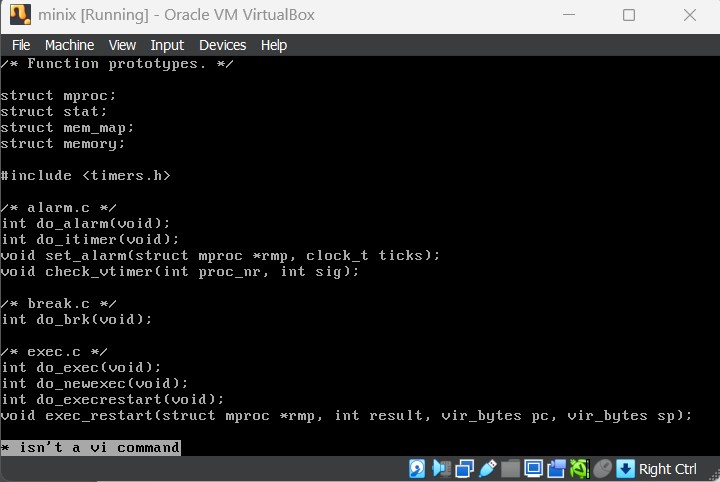
\includegraphics[scale=0.6]{out/fig/Screenshot 2024-12-23 113814}
    \caption{Conteúdo interno de \texttt{proto.h}.}
    \label{fig2}
\end{figure}

\subsection{Quinto Caso} \label{sec:5sec}
Agora é necessário através do comando de edição de arquivos \lstinline{vi}, devemos entrar dentro do arquivo \lstinline{misc.c} pelo caminho \lstinline{vi /usr/src/servers/pm/misc.c}.
Ao final do arquivo, deve-se inserir a função \ref{lst:code1}, conforme pode ser visto abaixo.

\begin{lstlisting}[caption={Programa em C que mostra o que faz a syscall}, label={lst:code1}, language=C]
     int do_minhachamada(void)
	{
		int input_number = m_in.m1_i1;
		printf("ola, sou a syscall inutil que imprime o numero % d na tela \n ", input_number);
		return 0;
	}
\end{lstlisting}

\subsection{Sexto Caso} \label{sec:6sec}

Dentro do arquivo \lstinline{/usr/src/servers/pm}, com o comando \lstinline{cd}, tente compilar o arquivo criado antes, digite \lstinline{make} e veja se o arquivo antes criado
está compilando de forma adequada. Lembrando que o sistema operacional Minix usa \lstinline{cc} como compilador C pré-instalado.

\subsection{Sétimo Caso} \label{sec:7sec}
De forma semelhante ao já realizado, com o comando \lstinline{vi}, no caminho \lstinline{/usr/include/mysyscalllib.h}, e adicione o código em \ref{lst:code2}. Após a finalização,
basta salvar o arquivo e passar para o próximo passo.

\begin{lstlisting}[caption={Programa em C para somar dois números}, label={lst:code2}, language=C]
    #include <lib.h>
	#include <unistd.h>
	int minhachamada(int n)
	{
		message m;
                          m.m1_i1 = n;
		return ( _syscall(PM_PROC_NR, MINHACHAMADA, &m) );
	}
\end{lstlisting}

Agora através do comando \lstinline{cd}, vá para o seguinte caminho \lstinline{/usr/src/releasetools}, e digite \lstinline{make install}. Após o comando anterior compilar
digite \lstinline{sync} e por fim reinicialize o sistema operacional com o comando \lstinline{reboot}. Caso ocorram erros ao final, por exemplo se ao reinicializar aparecer algum
erro, basta desligar e ligar novamente a máquina virtual.
\subsection{Oitavo caso}
Como último passo de alterações, vá para o diretório \texttt{root} e lá crie o arquivo C de testes com o conteúdo mostrado no código \ref{lst:code3}. Após finalizar a edição,
 assim como anteriormente, basta agora salvar e fechar o arquivo.
\begin{lstlisting}[caption={Programa em C para somar dois números}, label={lst:code3}, language=C]
    #include <mycalllib.h>
	int main(void)
	{
		int n = 10;
		minhachamada(n);
		return 0;
	}
\end{lstlisting}
Com o fim das alterações, agora é necessário compilar o arquivo de testes, então, através do comando de terminal que utiliza o compilador C, \lstinline{cc}, digite o seguinte
dentro do diretório onde o arquivo C criado está localizado. \lstinline{cc teste1.c -o test1.out} e depois compile o arquivo com o comando \lstinline{./test1.out}. Estando tudo
feito de forma adequada, ao final dessas alterações, a chamada de sistema deve funcionar de maneira adequada.


\subsection{Conclusão}

A implementação de uma syscall no sistema operacional Minix 3.2.1 proporcionou uma compreensão aprofundada sobre o funcionamento interno do kernel e o
processo de integração de novas funcionalidades no mesmo. Durante o desenvolvimento, explorei os principais arquivos e diretórios responsáveis por gerenciar as chamadas
de sistema, bem como as interações entre o kernel e o servidor de gerenciamento de processos.

A criação da syscall "inútil" demonstrou de forma prática como configurar, prototipar e testar uma funcionalidade personalizada. Além disso, o trabalho reforçou a
importância de ferramentas como o editor \texttt{vi}, comandos básicos de terminal e o compilador \texttt{cc}, que são indispensáveis para manipular sistemas baseados em Unix.

Este estudo serve como referência prática para desenvolvedores e estudantes interessados em sistemas operacionais, oferecendo um caminho claro para explorar os conceitos
fundamentais de syscalls e suas aplicações. Assim, contribui para o aprofundamento teórico e técnico no campo da Engenharia de Computação.

\bibliographystyle{sbc}

\newpage
\bibliography{sbc-template}



\end{document}
